\documentclass[11pt,a4paper]{article}
\usepackage[margin=1in]{geometry}
\usepackage[T1]{fontenc}
\usepackage[utf8]{inputenc}
\usepackage{lmodern}
\usepackage{hyperref}
\usepackage{enumitem}
\usepackage{xurl}
\usepackage{tikz}
\usepackage{float}
\usetikzlibrary{arrows.meta, positioning, shapes.geometric}
\hypersetup{colorlinks=true,linkcolor=blue,urlcolor=blue}
\newcommand{\codepath}[1]{\path{#1}}
\tikzset{
  box/.style={rectangle,draw,rounded corners,align=center,inner sep=3pt,minimum width=44mm},
  decision/.style={diamond,draw,aspect=2.2,align=center,inner sep=2pt},
  line/.style={-Latex}
}

\title{Phase-2 Spike: Deliverable 8 (Dataset Governance)}
\author{SIT Engine Documentation}
\date{\today}

\begin{document}
\maketitle

\section{Technical Description}
Spike dataset governance enforces provenance/version updates and deterministic replay checks for all baseline trace/mask changes.

\section{Implementation Fulfillment}
Governed assets are tracked in \codepath{Phase-2/datasets/}; governance checks use replay and determinism scripts before accepting dataset changes.

\section{Design \& Architecture}
\subsection*{Function Attributes}
\begin{itemize}[leftmargin=*]
  \item \texttt{build\_manifest()}: Inputs=trace/mask paths + metadata; Outputs=manifest JSON; Side effects=pins dataset version and replay inputs; Failure modes=incomplete metadata.
  \item \texttt{run\_golden\_suite.main()}: Inputs=manifest + output args; Outputs=replay pass/fail; Side effects=validates dataset replay correctness; Failure modes=replay failure.
  \item \texttt{check\_determinism.main()}: Inputs=targets + rerun configs; Outputs=determinism verdict; Side effects=guards against output drift; Failure modes=hash mismatch.
  \item \texttt{sha256\_file()}: Inputs=artifact path; Outputs=content hash; Side effects=tracks immutable dataset identity; Failure modes=file missing.
\end{itemize}
\subsection*{Function Execution Details}
\begin{enumerate}[leftmargin=*]
  \item \texttt{build\_manifest()}
  \begin{itemize}[leftmargin=*]
    \item Input attributes: trace/mask paths + metadata.
    \item Processing flow: pins dataset version and replay inputs.
    \item Output attributes: manifest JSON.
    \item Failure behavior: incomplete metadata.
  \end{itemize}
  \item \texttt{run\_golden\_suite.main()}
  \begin{itemize}[leftmargin=*]
    \item Input attributes: manifest + output args.
    \item Processing flow: validates dataset replay correctness.
    \item Output attributes: replay pass/fail.
    \item Failure behavior: replay failure.
  \end{itemize}
  \item \texttt{check\_determinism.main()}
  \begin{itemize}[leftmargin=*]
    \item Input attributes: targets + rerun configs.
    \item Processing flow: guards against output drift.
    \item Output attributes: determinism verdict.
    \item Failure behavior: hash mismatch.
  \end{itemize}
  \item \texttt{sha256\_file()}
  \begin{itemize}[leftmargin=*]
    \item Input attributes: artifact path.
    \item Processing flow: tracks immutable dataset identity.
    \item Output attributes: content hash.
    \item Failure behavior: file missing.
  \end{itemize}
\end{enumerate}


\subsection*{Diagram A: End-to-End Design Flow}
\begin{figure}[H]
\centering
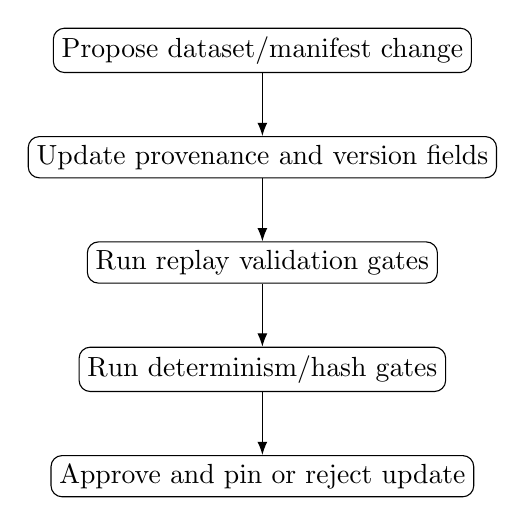
\begin{tikzpicture}[node distance=8mm and 12mm]
\node[box] (a) {Propose dataset/manifest change};
\node[box, below=of a] (b) {Update provenance and version fields};
\node[box, below=of b] (c) {Run replay validation gates};
\node[box, below=of c] (d) {Run determinism/hash gates};
\node[box, below=of d] (e) {Approve and pin or reject update};
\draw[line] (a) -- (b);
\draw[line] (b) -- (c);
\draw[line] (c) -- (d);
\draw[line] (d) -- (e);
\end{tikzpicture}
\caption{Spike Deliverable 08: End-to-End Design Flow}
\end{figure}

\subsection*{Diagram B: Function Interaction and Attribute Flow}
\begin{figure}[H]
\centering
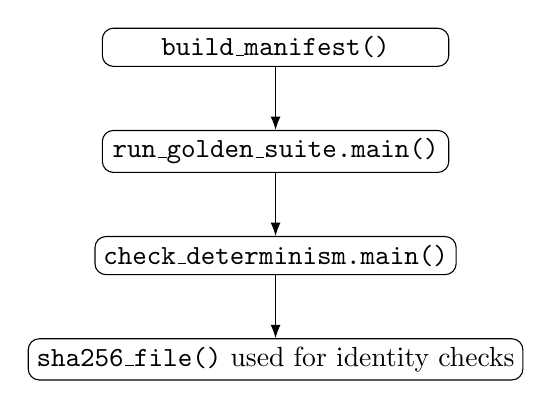
\begin{tikzpicture}[node distance=8mm and 12mm]
\node[box] (fa) {\texttt{build\_manifest()}};
\node[box, below=of fa] (fb) {\texttt{run\_golden\_suite.main()}};
\node[box, below=of fb] (fc) {\texttt{check\_determinism.main()}};
\node[box, below=of fc] (fd) {\texttt{sha256\_file()} used for identity checks};
\draw[line] (fa) -- (fb);
\draw[line] (fb) -- (fc);
\draw[line] (fc) -- (fd);
\end{tikzpicture}
\caption{Spike Deliverable 08: Function Interaction and Attribute Flow}
\end{figure}

\end{document}
